% THIS IS SIGPROC-SP.TEX - VERSION 3.1
% WORKS WITH V3.2SP OF ACM_PROC_ARTICLE-SP.CLS
% APRIL 2009
%
% It is an example file showing how to use the 'acm_proc_article-sp.cls' V3.2SP
% LaTeX2e document class file for Conference Proceedings submissions.
% ----------------------------------------------------------------------------------------------------------------
% This .tex file (and associated .cls V3.2SP) *DOES NOT* produce:
%       1) The Permission Statement
%       2) The Conference (location) Info information
%       3) The Copyright Line with ACM data
%       4) Page numbering
% ---------------------------------------------------------------------------------------------------------------
% It is an example which *does* use the .bib file (from which the .bbl file
% is produced).
% REMEMBER HOWEVER: After having produced the .bbl file,
% and prior to final submission,
% you need to 'insert'  your .bbl file into your source .tex file so as to provide
% ONE 'self-contained' source file.
%
% Questions regarding SIGS should be sent to
% Adrienne Griscti ---> griscti@acm.org
%
% Questions/suggestions regarding the guidelines, .tex and .cls files, etc. to
% Gerald Murray ---> murray@hq.acm.org
%
% For tracking purposes - this is V3.1SP - APRIL 2009

\documentclass{acm_proc_article-sp}

\begin{document}

% set the path for graphics
\graphicspath{{figures/}}

\title{User-Device Physical Unclonable Functions (UD-PUFs) based on Mobile Device Touchscreen Pressure}
%\subtitle{[Extended Abstract]
%\titlenote{A full version of this paper is available as
%\textit{Author's Guide to Preparing ACM SIG Proceedings Using
%\LaTeX$2_\epsilon$\ and BibTeX} at
%\texttt{www.acm.org/eaddress.htm}}}
%
% You need the command \numberofauthors to handle the 'placement
% and alignment' of the authors beneath the title.
%
% For aesthetic reasons, we recommend 'three authors at a time'
% i.e. three 'name/affiliation blocks' be placed beneath the title.
%
% NOTE: You are NOT restricted in how many 'rows' of
% "name/affiliations" may appear. We just ask that you restrict
% the number of 'columns' to three.
%
% Because of the available 'opening page real-estate'
% we ask you to refrain from putting more than six authors
% (two rows with three columns) beneath the article title.
% More than six makes the first-page appear very cluttered indeed.
%
% Use the \alignauthor commands to handle the names
% and affiliations for an 'aesthetic maximum' of six authors.
% Add names, affiliations, addresses for
% the seventh etc. author(s) as the argument for the
% \additionalauthors command.
% These 'additional authors' will be output/set for you
% without further effort on your part as the last section in
% the body of your article BEFORE References or any Appendices.

\numberofauthors{3} %  in this sample file, there are a *total*
% of EIGHT authors. SIX appear on the 'first-page' (for formatting
% reasons) and the remaining two appear in the \additionalauthors section.
%
\author{
% 1st. author
\alignauthor Timothy M. Dee\\
       \affaddr{Electrical \& Computer Engineering}\\
       \affaddr{Iowa State University}\\
       \affaddr{Ames, IA, USA}\\
       \email{deetimothy33@gmail.com}
% 2nd. author
%\alignauthor Ian T. Richardson\\
%       \affaddr{Electrical \& Computer Engineering}\\
%       \affaddr{Iowa State University}\\
%       \affaddr{Ames, IA, USA}\\
%       \email{ian.t.rich@gmail.com}
% 3nd. author
\alignauthor Akhilesh Tyagi\\
      \affaddr{Electrical \& Computer Engineering}\\
      \affaddr{Iowa State University}\\
       \affaddr{Ames, IA, USA}\\
       \email{tyagi@iastate.edu}
}

%\date{30 July 1999}
% Just remember to make sure that the TOTAL number of authors
% is the number that will appear on the first page PLUS the
% number that will appear in the \additionalauthors section.

\maketitle
\begin{abstract}
%TODO remove the last sentence, mabe?
Described in this document is a physical unclonable function (PUF) utilizing the variability derived from the pressure with which users interact with their mobile device touchscreens. We illustrate how a sequence of these pressure values from descrete touchscreen interactions may be used to uniquely characterize a user-device pair. This characterization method may find many applications in protecting access to a mobile device from a malicious party. As a result, the effectiveness of this scheme is described in terms of how one user may be differentiated from another.
\end{abstract}

% A category with the (minimum) three required fields
%\category{H.4}{Information Systems Applications}{Miscellaneous}
%A category including the fourth, optional field follows...
%\category{D.2.8}{Software Engineering}{Metrics}[complexity measures, performance measures]

%\terms{Theory}

%\keywords{physical unclonable function (PUF), mobile device authentication} % NOT required for Proceedings

\section{Introduction}
\label{sec:intro}
Mobile devices are ubiquitus in the modern world. These devices are becoming progressively more important for many applications with security sensative data. 
Securing mobile devices poses unique challenges and opportunities compared to traditional data security where it is difficult for an attacker to access the physical device on which the data is stored or from which the sensitive data may be accessed.
%
The reality that an attacker may be able to gain access to a physical device makes securing any data stored on or accessed by a mobile device significantly more challenging. Traditional physical unclonable functions (PUFs) which can be used to uniquely to a given hardware device are no longer sufficient to guarentee the authenticity of a user.
%
This modivates an extension of the traditional PUF known as a user-device physical unclonable function(UD-PUF). This UD-PUF entangles the physical characteristics of the user in combination with the device to enable a more secure authentication scheme.

%describe what touchscreen pressure is
%describe the physical component of the pressure (current at the edge of screen on android device)
\section{Touchscreen Pressure}
\label{sec:touchscreen}
%TODO 
current at sides of phone.\cite{zhu2013sensec}

%describe a marcov model in general
%describe what it means to be an n-gram sliding marcov model
%describe in what way we a marcov model to describe a user, device pair (our marcov model of touch, pressure values.
%An n-gram sliding marcov model.
\section{Modeling a User-Device Pair}
\label{sec:modeling}
Interactions between useres and devices are complex. To interpret these actions in a meaningful way, in order to preform an authentication for example, it is necessary to simplify these interations. The chosen model must provide sufficient entropy such that a model generated with a given user-device pair is not consistantly reproducable by another user or on a different device. The modeling method must also be easily reproducable by the origional user on the origional device. A model having the neccessary characteristics required for this application is a Marcov Chain.
%
%TODO describe what is a marcov chain
Marcov Chains are useful in predicting systems who's behavior can be modeled in descrete states. The transitions between states can be identified to happen with some probability.
%Other information about marcov chains
%TODO traditional use of marcov chains
Historically the Marcov Chain has found applications in
%
Upon identification of an appropriate model the next step is to discover an optimal way in which it may be applied to the current problem. The goal is %TODO
%


%n-gram a continuious sequence of n items
%markov model for comparason is built from a sliding model of the previous n touches
%describe how the marcov chain is applied to touch pressure to model a user
%this is a description of our specific implementation of a marcov model
\section{Touch Pressure Modeling}
%TODO
%describe the marcov model used
%
The goal in modeling a system with a marcov model is to classify the system in terms of its transitions between states. If such a model is to be used to purposes of uniquely identifying a given system, than the states of the model must be chosen in a way which exposes the uniqueness of the system.
The states of our marcov model are defined by the range in which


%basically the authentication scheme used
%frame it in more general terms, independtant of our specific application
\section{Differentiating User-Device Pairs}
\label{sec:differentiation}

\begin{figure}
\centering
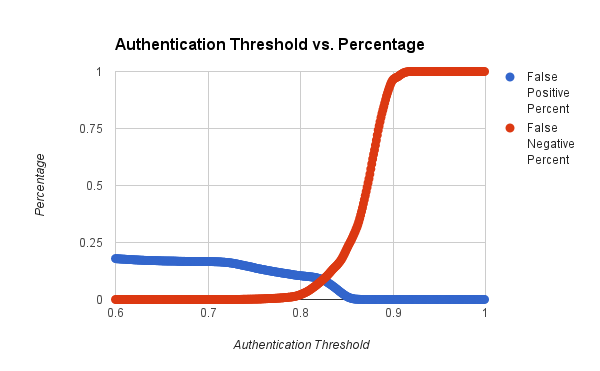
\includegraphics[width=3.9in]{threshold_vs_percentages.png}
\caption{TODO}
\label{fig:threshold_vs_percentages}
\end{figure}

%what number of states exposed the most uniqueness e.g. how many tokens were best
%with what accuracy could users be destinguished from one-another
\section{Results}
\label{sec:results}


\section{Conclusions}
\label{sec:conclusions}


%possible, describe applications  in terms of continuious authentication
\section{Future Work}
\label{sec:futurework}

\bibliographystyle{abbrv}
\bibliography{bibliography/marcov_chains,bibliography/pufs,bibliography/other}
\end{document}
